% ---- pg-554 （书页 542） ----

水、土壤、小气候、温度甚至空气质量等因素的影响.” \hfill$\blacksquare$

\mvsub{对分层方法的最后评注}

除了单连接、完全连接和平均连接之外, 还有许多聚集型分层聚类方法. 然而, 所有聚集型方法都遵循式(12-12) 中的基本算法.

同大多数聚类方法一样, 在分层方法中, 误差和变差来源并未得到正式考虑. 这就意味着聚类方法对离群值或“噪音点”很敏感.

在分层聚类中, 对于那些在早期阶段被“错误”分组的对象不提供重新分组的机会. 因此, 始终应对最终的聚类结构进行仔细检查, 看看结果是否合情合理.

对某个特定的问题, 较好的做法是试用几种聚类方法, 而对一种给定的方法, 可以试用几种不同的距离(相似性).
如果用几种不同方法得到的结果(大体上)彼此一致, 那么就有可能找到一个“自然”分组.

某个分层解的稳定性有时可用这样的方法来检查: 对数据单元加进一些小误差(干扰), 然后运用聚类算法, 并将新的结果与未加误差时的结果进行比较.
如果各组数据能很好区分, 则两种结果应大体吻合.

距离矩阵或相似性矩阵中的相同值(结)有可能使分层聚类问题产生多重解. 也就是说, 用不同方法处理打结的相似性(距离)会得出不同的树图, 特别是在较低的水平上.
并非任何方法都会出现这种问题, 只有特定类型的数据才会发生多重解. 出现多重解未必是坏事.
不过聚类方法的应用者应该知道这种现象的存在, 以便对分组(树图)给出恰当的解释, 并比较不同的分组(树图), 以评估它们的重合程度.
对这个问题的进一步讨论可在文献[27]中找到.

某些数据集和分层聚类方法会产生“逆序”(见文献[27]).
当某个对象在并入一个已有的聚类时其距离小于上一次合并的距离, 就会发生逆序. 在下图中, 用两种不同方法代表一个逆序.

\begin{mvfigure}
\begin{minipage}[t]{0.44\linewidth}\centering
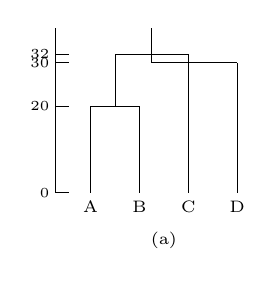
\begin{tikzpicture}[x=0.62cm,y=0.055cm,line width=0.4pt]
% 坐标轴
\draw (-0.72,0) -- (-0.72,38);
\draw (-0.72,0)  -- (-0.45,0);   \node[anchor=east,font=\fontsize{5}{6}\selectfont,inner sep=1pt] at (-0.78,0)  {0};
\draw (-0.72,20) -- (-0.45,20);  \node[anchor=east,font=\fontsize{5}{6}\selectfont,inner sep=1pt] at (-0.78,20) {20};
\draw (-0.72,30) -- (-0.45,30);  \node[anchor=east,font=\fontsize{5}{6}\selectfont,inner sep=1pt] at (-0.78,30) {30};
\draw (-0.72,32) -- (-0.45,32);  \node[anchor=east,font=\fontsize{5}{6}\selectfont,inner sep=1pt] at (-0.78,32) {32};
% 树图
\draw (0,0) -- (0,20);
\draw (1,0) -- (1,20);
\draw (0,20) -- (1,20);
\draw (0.5,20) -- (0.5,32);
\draw (0.5,32) -- (2,32);
\draw (1.25,32) -- (1.25,30);
\draw (1.25,30) -- (3,30);
\draw (1.25,32) -- (1.25,38);
\draw (2,0) -- (2,32);
\draw (3,0) -- (3,30);
% 叶子
\foreach \i/\lb in {0/A,1/B,2/C,3/D} {
  \node[font=\fontsize{6}{7}\selectfont,inner sep=1pt,anchor=north,yshift=-2pt] at (\i,0) {\lb};
}
\node[font=\fontsize{6}{7}\selectfont,inner sep=4pt] at (1.5,-11) {(a)};
\end{tikzpicture}
\end{minipage}\hfill
\begin{minipage}[t]{0.44\linewidth}\centering
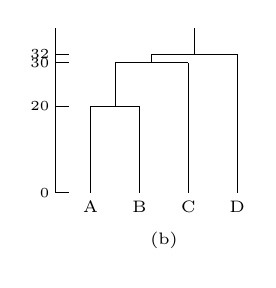
\begin{tikzpicture}[x=0.62cm,y=0.055cm,line width=0.4pt]
% 坐标轴
\draw (-0.72,0) -- (-0.72,38);
\draw (-0.72,0)  -- (-0.45,0);   \node[anchor=east,font=\fontsize{5}{6}\selectfont,inner sep=1pt] at (-0.78,0)  {0};
\draw (-0.72,20) -- (-0.45,20);  \node[anchor=east,font=\fontsize{5}{6}\selectfont,inner sep=1pt] at (-0.78,20) {20};
\draw (-0.72,30) -- (-0.45,30);  \node[anchor=east,font=\fontsize{5}{6}\selectfont,inner sep=1pt] at (-0.78,30) {30};
\draw (-0.72,32) -- (-0.45,32);  \node[anchor=east,font=\fontsize{5}{6}\selectfont,inner sep=1pt] at (-0.78,32) {32};
% 树图
\draw (0,0) -- (0,20);
\draw (1,0) -- (1,20);
\draw (0,20) -- (1,20);
\draw (0.5,20) -- (0.5,30);
\draw (0.5,30) -- (2,30);
\draw (1.25,30) -- (1.25,32);
\draw (1.25,32) -- (3,32);
\draw (2.125,32) -- (2.125,38);
\draw (2,0) -- (2,30);
\draw (3,0) -- (3,32);
% 叶子
\foreach \i/\lb in {0/A,1/B,2/C,3/D} {
  \node[font=\fontsize{6}{7}\selectfont,inner sep=1pt,anchor=north,yshift=-2pt] at (\i,0) {\lb};
}
\node[font=\fontsize{6}{7}\selectfont,inner sep=4pt] at (1.5,-11) {(b)};
\end{tikzpicture}
\end{minipage}
\end{mvfigure}

在此例中, A 和 B 在距离 20 处合并. 下一步, C 在距离 32 处被加进(AB)组.
由于聚类算法的性质, D 在距离 30 处被加进(ABC)组. 这个距离小于 C 被加进(AB)组时的距离.
在图 (a) 中, 逆序由一个带交叉的树图表示. 在图 (b) 中, 逆序由一个具有非单调尺度的树图表示.

在没有清晰的聚类结构的情况下, 就会出现逆序, 因此逆序一般与两种分层聚类算法(即中心方法和中位数方法)相联系.
本书中所讨论的分层方法不易产生逆序.

\section{非分层聚类方法}
\phantomsection\label{sec:12.4}

设计非分层聚类技术的目的是, 为了将项目(不是变量)分成由 $K$ 个聚类组成的集合.
聚类的个数 $K$ 可以事先指定, 也可以在聚类过程中确定. 由于在计算机运行过程中不必确定距
